\lab{The Discrete Fourier Transform}{The Discrete Fourier Transform}
\objective{The analysis of periodic functions has many applications in pure and applied mathematics, especially in settings dealing with sound waves.
The Fourier transform provides a way to analyze such periodic functions.
In this lab, we use Python to work with digital audio signals and implement the discrete Fourier transform.
We use the Fourier transform to detect frequencies present in a given sound wave.
We recommend this lab be done in a Jupyter Notebook.}

\section*{Sound Waves} % ======================================================

Sound is how vibrations are perceived in matter.
These vibrations travel in waves.
Sound waves have two important characteristics that determine what is heard, or whether or not it can be heard.
The first characteristic is \emph{frequency}, which is a measurement of the number of vibrations in a certain time period, and determines the pitch of the sound.
Only certain frequencies are perceptible to the human ear.
The second characteristic is \emph{intensity} or \emph{amplitude}, and determines the volume of the sound.
Sound waves correspond physically to continuous functions, but computers can approximate sound waves using discrete measurements.
Indeed, discrete measurements can be made indistinguishable to the human ear from a truly continuous wave.
Usually, sound waves are of a sinusoidal nature (with some form of decay); the frequency is related to the wavelength, and the intensity to the wave amplitude.

\section*{Digital Audio Signals} % ============================================

Computer use \emph{digital audio signals} to approximate sound waves.
These signals have two key components that relate to the frequency and amplitude of sound waves: samples and sampling rate.
A sample is a measurement of the amplitude of a sound wave at a specific instant in time.
The sampling rate corresponds to the sound frequency.

To see why the sample rate is necessary, consider an array with samples from a sound wave.
If how frequently those samples were collected is unknown, then the sound wave can be arbitrarily stretched or compressed to make a variety of sounds.
See Figure \ref{fig:comp_wave} for an illustration of this principle.
\begin{figure}
\captionsetup[subfigure]{justification=centering}
\centering
\begin{subfigure}{.4\textwidth}
    \centering
    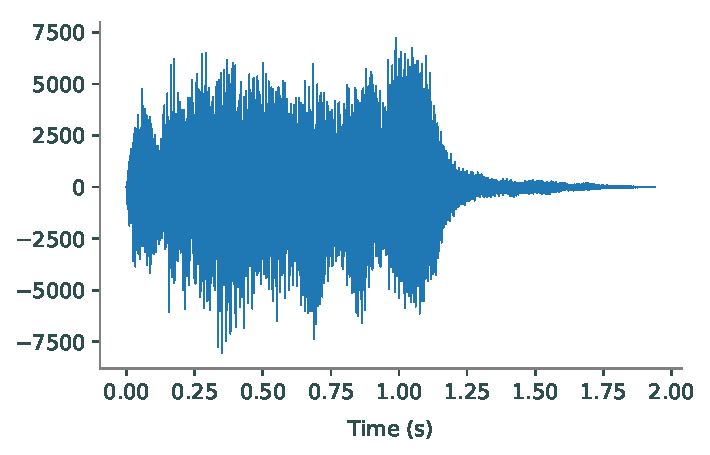
\includegraphics[width=\linewidth]{figures/tada.pdf}
    \caption{The plot of \texttt{tada.wav}.}
    \label{fig:tada}
\end{subfigure}
\begin{subfigure}{.4\textwidth}
    \centering
    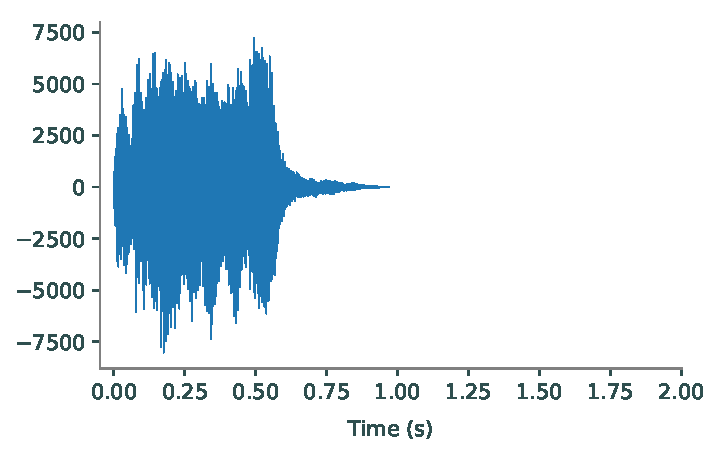
\includegraphics[width=\linewidth]{figures/fast_tada.pdf}
    \caption{Compressed plot of \texttt{tada.wav}}
    \label{fig:fasttada}
\end{subfigure}
\label{fig:comp_wave}
\caption{The plots of the same set of samples from a sound wave with varying sample rates.
The plot on the left is the plot of the samples with the original sample rate (in this case, 22050), while the sample rate of the plot on the right has been doubled, resulting in a compression of the actual sound when played back.
The compressed sound will be shorter and have a higher pitch.
Similarly, if this set of samples were played back with a lower sample rate will be stretched and have a lower pitch.}
\end{figure}

However, if the rate at which a set of samples is taken is known, the wave can be reconstructed exactly as it was recorded.
If the sample rate is unknown, then the frequencies will be unknown.
In most applications, this sample rate will be measured in the number of samples taken per second, Hertz (Hz).
The standard rate for high quality audio is $44100$ equally spaced samples per second, or $44.1$ kHz.

\subsection*{Wave File Format} % ----------------------------------------------

One of the most common audio file formats across operating systems is the \emph{wave} format, also called \texttt{wav} after its file extension.
SciPy has built-in tools to read and create \texttt{wav} files.
To read in a \texttt{wav} file, use SciPy's \li{read()} function that returns the file's sample rate and samples.

\begin{lstlisting}
# Read from the sound file.
>>> from scipy.io import wavfile
>>> rate, wave = wavfile.read('tada.wav')
\end{lstlisting}

It is sometimes useful to visualize a sound wave by plotting time against the amplitude of the sound, as in Figure \ref{fig:comp_wave}.
This type of plotting plots in the \emph{time domain}.
The amplitude of the sound at a given time is just the value of the sample at that time.
Note that since the sample rate is given in samples per second, the length of the sound wave in seconds is found by dividing the number of samples by the sample rate.

% Problem 1: SoundWave class
\begin{problem}
Make a class called \li{SoundWave} for storing digital audio signals.
Write the constructor and have it accept a sample rate (integer) and an array of samples (NumPy array), which it stores as class attributes.
Then, write a method called \li{plot()} that generates the graph of the sound wave.
Use the sample rate to label the x-axis in terms of seconds.
Finally, construct a \li{SoundWave} object using the data in \texttt{tada.wav} and display its plot.
Your plot should look like Figure \ref{fig:tada}.
\end{problem}

\subsection*{Scaling} % -------------------------------------------------------

Writing a sound wave to a file is slightly more complicated than reading from a file.
Use \li{wavfile.write()}, specifying the name of the new file, the sample rate, and the array of samples.

\begin{lstlisting}
# Write a random signal sampled at a rate of 44100 Hz to my_sound.wav.
>>> wave = np.random.randint(-32767, 32767, 30000)
>>> samplerate = 44100
>>> wavfile.write('my_sound.wav', samplerate, wave)
\end{lstlisting}

In order for the \li{wavfile.write()} function to accurately write an array of samples to a file, the samples must be of an appropriate type.
There are four types of sample values that the function will accept: 32-bit floating point, 32-bit integers, 16-bit integers, and 8-bit unsigned integers.
If a different type of samples are passed into the function, it's possible that the function will write to a file, but the sound will likely be distorted in some way.
This lab works with only 16-bit integer types, unless otherwise specified.

\begin{lstlisting}
# The type of the elements of an array is stored in an attribute called dtype.
>>> x = np.array([1, 2, 3])
>>> y = np.array([1.0, 2.0, 3.0])
>>> print(x.dtype)
dtype('int64')
>>> print(y.dtype)
dtype('float64')
\end{lstlisting}

A 16-bit integer is an integer between $-32767$ and $32767$.
If an array of samples does not already have all of its elements as 16-bit integers, it will need to be scaled in such a way so that is does before it can be written to a file.
In addition, it is ideal to scale the samples so that they cover as much of the 16-bit integer range as possible.
This will ensure the most accurate representation of the sound.

\begin{lstlisting}
# Generate random samples between -0.5 and 0.5.
>>> samples = np.random.random(30000)-.5
>>> print(samples.dtype)
dtype('float64')
# Scale the wave so that the samples are between -32767 and 32767.
>>> samples *= 32767*2
# Cast the samples as 16-bit integers.
>>> samples = np.int16(samples)
>>> print(samples.dtype)
dtype('int16')
\end{lstlisting}

In the above example, the original samples are all less than $0.5$ in absolute value.
Multiplying the original samples by $32767$ and $2$ scales the samples appropriately.
In general, to get the scaled samples from the original, multiply by $32767$ and divide by the greatest magnitude present in the original sample.
Note also that for various reasons, samples may sometimes contain complex values.
In this case, scale and export only the real part.

% Problem 2: Signal.export
\begin{problem}
Add a method to the \li{SoundWave} class called \li{export()} that accepts a file name and generates a \texttt{.wav} file of that name from the sample rate and the array of samples.
If the array of samples is not already in \texttt{int16} format, scale it appropriately before writing to the output file.
Use your method to create a differently named file that contains the same sound as \texttt{tada.wav}.
Display the two sounds to make sure the method works correctly.
\begin{info}
To display a sound in a Jupyter Notebook, first import IPython, then use \li{IPython.display.Audio()}.
This function can accept either the name of a \texttt{.wav} file present in the same directory, or the keyword arguments \texttt{rate} and \texttt{data}, which represent the sample rate and the array of samples, respectively.
The function will generate a music player that can be played within the Jupyter Notebook.
\end{info}
\end{problem}

\section*{Creating Sounds in Python} % ========================================

In order to generate a sound in Python, sample the corresponding sinusoidal wave.
The example below generates a sound with a frequency of 500 Hertz for 10 seconds.

\begin{lstlisting}
>>> samplerate = 44100
>>> frequency = 500.0
>>> duration = 10.0         # Length in seconds of the desired sound.
\end{lstlisting}

Recall the the function $\sin(x)$ has a period of $2\pi$.
To create sounds, however, the desired period of a wave is $1$, corresponding to $1$ second.
Thus, sample from the function
\[
\sin(2\pi xk)
\]
where $k$ is the desired frequency.

\begin{lstlisting}
# The lambda keyword is a shortcut for creating a one-line function.
>>> wave_function = lambda x: np.sin(2*np.pi*x*frequency)
\end{lstlisting}

To generate a sound wave, use the following three steps:
First, generate the points at which to sample the wave.
Next, sample the wave by passing the sample points into \li{wave_function()}.
Then, use the \li{SoundWave} class to plot the sound wave or write it to a file.

\begin{lstlisting}
# Calculate the sample points and the sample values.
>>> sample_points = np.linspace(0, duration, int(samplerate*duration))
>>> samples = wave_function(sample_points)

# Use the SoundWave class to write the sound to a file.
>>> sound = SoundWave(samplerate, samples)
>>> sound.export("example.wav")
\end{lstlisting}

\begin{comment}
In this case, the samples are numbers between 0 to 1, taken from \li{wave_function()}.
However, \li{wavfile.write()} requires integers between $-32767$ and $32767$.
Thus, we scale our sample points before creating a \texttt{.wav} file that can be played by the computer.

\begin{lstlisting}
>>> scaled_samples = sp.int16(samples*32767)
\end{lstlisting}

The \li{scaled_samples} array can now be written to a file using \li{wavfile.write()}.
This file can be played using media software included with most operating systems.
\end{comment}

% Problem 3: make a sound.
\begin{problem}
Write a function that accepts a frequency and a duration.
Follow the pattern above to generate and return an instance of the SoundWave class with the given frequency and duration.
Use a sample rate of 44100.

The following table shows some frequencies that correspond to common notes.
Octaves of these notes are obtained by doubling or halving these frequencies.

\begin{center}
\begin{tabular}{|c|c|}
\hline
Note & Frequency \\
\hline
A & 440 \\
B & 493.88 \\
C & 523.25 \\
D & 587.33 \\
E & 659.25 \\
F & 698.46 \\
G & 783.99 \\
A & 880 \\
\hline
\end{tabular}
\end{center}

The ``A'' note occurs at a frequency of 440 Hertz.
Use your function to generate and display an ``A'' note being played for 2 seconds.
\label{prob:generate_note}
\end{problem}

% Problem 4: make a chord and a changing sound.
\begin{problem}
\leavevmode
\begin{enumerate}
\item A chord is a conjunction of several notes played together.
You can create a chord in Python by adding several sound waves together.
Write the \li{__add__()} magic method in the SoundWave so that it adds together the samples of two \li{SoundWave} objects and returns the resulting \li{SoundWave} object.
Note this is only valid if the two sample arrays are the same length.
Raise a \li{ValueError} if the arrays are not the same length.
\item Generate and display a minor chord (made up of the ``A'', ``C'', and ``E'' notes).
\item Add a method called \li{append()} to the \li{SoundWave} class that accepts a \li{SoundWave} object and appends the additional samples from the new object to the end of the samples from the current object.
Note this only makes sense if the sample rates of the two objects are the same.
Raise a \li{ValueError} if the sample rates of the two objects are not equal.
\item Finally, generate and display a sound that changes over time.

\end{enumerate}
\end{problem}

\section*{Discrete Fourier Transform} % =======================================

Under the right conditions, a continuous periodic function may be represented as a sum of sine waves:
\[
f(x) = \displaystyle{\sum_{k=-\infty}^{\infty}} c_k \sin{kx}
\]
where the constants $c_k$ are called the \emph{Fourier coefficients}.

Such a transform also exists for discrete periodic functions.
Whereas the frequencies present in the continuous case are multiples of a sine wave with a period of 1, the discrete case is somewhat different.
The Fourier coefficients in the discrete case represent the amplitudes of sine waves whose periods are multiples of a ``fundamental frequency''.
The fundamental frequency is a sine wave with a period length equal to the amount of time of the sound wave.

The $k^{th}$ coefficient of a sound wave $\{x_0, .., x_{N-1}\}$ is calculated with the following formula:
\begin{align}
c_k = \displaystyle{\sum_{n=0}^{N-1}} x_n e^{\frac{-2\pi ikn}{N}}\label{eq:ck}
\end{align}
where $i$ is the square root of $-1$.
This process is done for each $k$ from $0$ to $N-1$, where $N$ is the number of sample points.
Thus, there are just as many Fourier coefficients as samples from the original signal.
The discrete Fourier transform (DFT) is particularly useful when dealing with sound waves.
The applications will be discussed further later on in the lab.

% Problem 5: Naive DFT
\begin{problem} 
Write a function called \li{naive_DFT()} that accepts a NumPy array and computes the discrete Fourier transform of the array using Equation \ref{eq:ck}.
Return the array of calculated coefficients.

SciPy has several methods for calculating the DFT of an array.
Use \li{scipy.fft()} or \li{scipy.fftpack.fft()} to check your implementation by using your method and the SciPy method to calculate the DFT and comparing the results using \li{np.allclose()}.
The naive method is significantly slower than SciPy's implementation, so test your function only on small arrays.
When you have your method working, try to optimize it so that you can calculate each coefficient $c_k$ in just one line of code.
\label{prob:dft}
\end{problem}

\section*{Fast Fourier Transform}

Calculating the DFT of a large set of samples using only (\ref{eq:ck}) can be incredibly slow.
Fortunately, when the size of the samples is a power of $2$, the DFT can be implemented as a recursive algorithm by separating the computation of the DFT into its even and odd indices.
This method of calculating the DFT is called the \emph{Fast Fourier Transform} (FFT) due to its remarkably improved run time. 
The following algorithm is a simple implementation of the FFT.

\begin{algorithm}[H]
\begin{algorithmic}[1]
\Procedure{FFT}{$x$}
    \State $N \gets \size{x}$
    \If{$N = 1$}
        \State \pseudoli{return} DFT($x$)
            \Comment{Use the DFT function you wrote for Problem \ref{prob:dft}.}
    \Else{}
        \State $even \gets$ FFT($x_{::2}$)
        \State $odd \gets$ FFT($x_{1::2}$)
        \State $k \gets arange(N)$
            \Comment{Use \li{np.arange}.}
        \State $factor \gets exp(-2 \pi ik / N)$
        \State 
            \Comment{Note $*$ is component-wise multiplication.}
        \State \pseudoli{return} $concatenate((even + factor_{:N/2} * odd, even + factor_{N/2:} * odd))$
        \EndIf
\EndProcedure
\end{algorithmic}
\caption{}
\label{alg:FFT}
\end{algorithm}

This algorithm performs significantly better than the naive implementation using only (\ref{eq:ck}).
However, this simplified version will only work if the size of the input samples is exactly a power of $2$.
SciPy's FFT functions manage to get around this by padding the sample array with zeros until the size is a power of $2$, then executing the remainder of the algorithm from there.
In addition, SciPy's functions use various other tricks to speed up the algorithm even further.

% Problem 6: FFT - implement by hand, time / compare with SciPy
\begin{problem}
Write a function that accepts a NumPy array and computes the discrete Fourier transform of the array using Algorithm \ref{alg:FFT}. 
Return the array of calculated coefficients.

To verify your method works, generate an array of random samples of a size that is a power of 2 (preferably size 1024 or larger) and use \li{np.allclose()} as in the previous problem to make sure the outputs are the same.
Then, compare the runtimes of your DFT method, your FFT method, and one of the SciPy methods and print the results.

Hint: Concatenating vectors can be done with \li{np.concatenate}.
\end{problem}

\section*{Plotting the DFT} % =================================================

\begin{figure}
\captionsetup[subfigure]{justification=centering}
\centering
\begin{subfigure}{.4\textwidth}
    \centering
    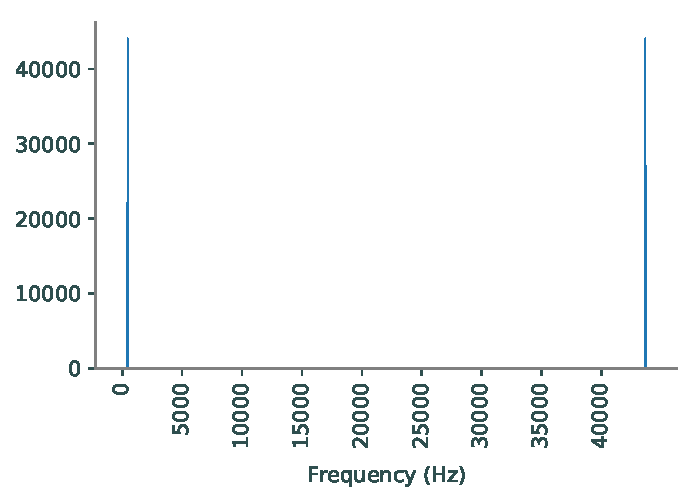
\includegraphics[width=\linewidth]{figures/dft_a.pdf}
    \caption{The DFT of the ``A'' note (with symmetries).}
    \label{fig:dft_a}
\end{subfigure}
\begin{subfigure}{.4\textwidth}
    \centering
    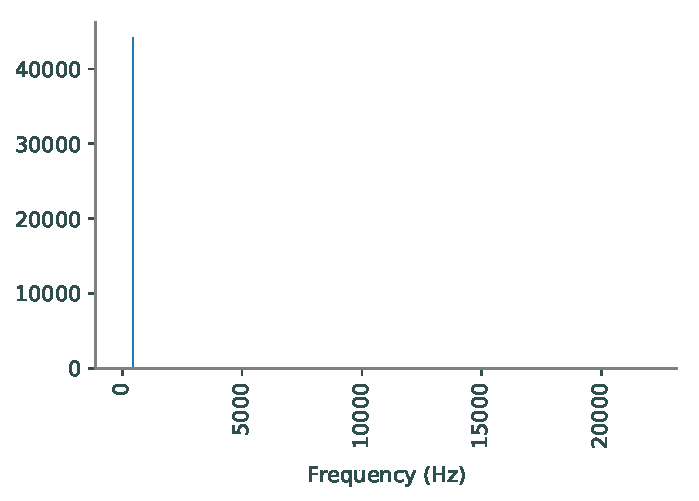
\includegraphics[width=\linewidth]{figures/dft_a_half.pdf}
    \caption{The DFT of the ``A'' note (without symmetries).}
    \label{fig:dft_a_half}
\end{subfigure}
\label{fig:DFTs}
\caption{Plots of the DFT (with and without symmetries).
Notice that the x-axis of the symmetrical plot goes up to $44100$, or the sample rate of the sound wave being plotted, while the x-axis of the other plot goes up to half of that.
Also notice that the spikes occur at $440.0$ Hz and $43660.0$ Hz (which is $44100.0 - 440.0$).}
\end{figure}

The graph of the Fourier transform of a sound file is useful in a variety of applications.
While the graph of the sound in the time domain gives information about the amplitude of a sound wave at a given time, the graph of the discrete Fourier transform shows which frequencies are present in the signal.
Plotting a sound's DFT is referred to as plotting in the \emph{frequency domain}.
Often, this information is of greater importance.

Frequencies present in the sound have non-zero coefficients.
The magnitude of these coefficients corresponds to how influential the frequency is in the signal.
For example, in the case of the ``A'' note in Problem \ref{prob:generate_note} the sound contained only one frequency.
The graph of the DFT of this sound is Figure \ref{fig:dft_a}.
% However, there is a catch.
Note that in this plot, there are two spikes, despite there being only one frequency present in the sound.
This is due to symmetries inherent in the DFT.
For the purposes of this lab, ignore the second half of the plot.
From now on, show plots of only the first half of the DFT, as in Figure \ref{fig:dft_a_half}.

On the other hand, the DFT of a more complicated sound wave will have many frequencies present.
Some of these frequencies correspond to the different tones present in the signal.
See Figure \ref{fig:dft_tada} for an example.

\begin{center}
\begin{figure}
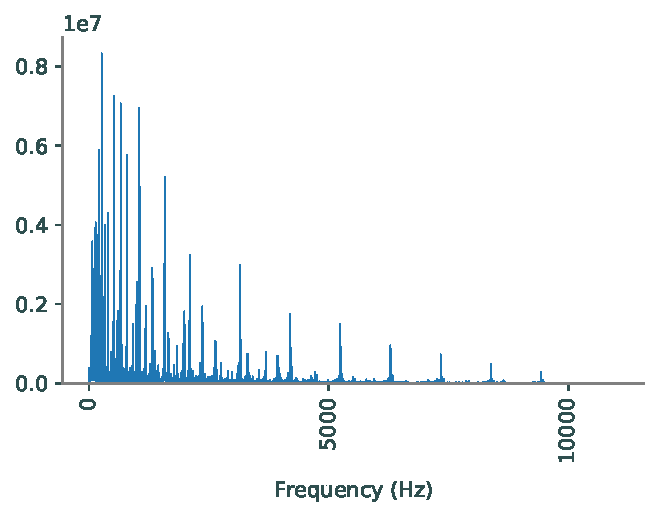
\includegraphics[scale=1.0]{figures/dft_tada.pdf}
\caption{The discrete Fourier transform of \texttt{tada.wav}.
Each spike in the graph corresponds to a frequency present in the signal.
Since the sample rate of \texttt{tada.wav} is only $22050$ instead of the usual $44100$, the plot of its DFT without symmetries will only go up to $11025$, half of its sample rate.} 
\label{fig:dft_tada}
\end{figure}
\end{center}

\subsection*{Fixing the x-axis} % ---------------------------------------------

Plotting the DFT of a signal without any other considerations results in an x-axis that corresponds to the index of the coefficients in the DFT, not their frequencies.
As mentioned earlier, the ``fundamental frequency'' for the DFT corresponds to a sine wave whose period is the same as the length of the signal.
Thus, if unchanged, the x-axis gives the number of times a particular sine wave cycles throughout the whole signal.
To label the x-axis with the frequencies measured in Hertz, or cycles per second, the units must be converted.
Fortunately, the bitrate is measured in samples per second.
Therefore, dividing the frequency (given by the index) by the number of samples and multiplying by the sample rate, results in cycles per second, or Hertz.

\begin{center}
    $\frac{\mbox{cycles}}{\mbox{samples}} \times \frac{\mbox{samples}}{\mbox{second}} = \frac{\mbox{cycles}}{\mbox{second}}$
\end{center}

\begin{lstlisting}
# Calculate the DFT and the x-values that correspond to the coefficients. Then
# convert the x-values so that they measure frequencies in Hertz.
>>> dft = abs(sp.fft(samples))       # Ignore the complex part.
>>> N = dft.shape[0]
>>> x_vals = np.linspace(1, N, N)
>>> x_vals = x_vals * samplerate / N # Convert x_vals to frequencies
\end{lstlisting}

% Problem 7: plotting the DFT.
\begin{problem}
Write a method in the \li{SoundWave} class called \li{plot_dft()} that plots the frequencies present in a sound wave on the x-axis and the magnitude of those frequencies on the y-axis. 
Only display the first half of the plot (as in Figure \ref{fig:dft_a_half}).
Use one of SciPy's FFT implementations to calculate the DFT.

Display the DFT plots of the `A' note and of the minor chord.
\end{problem}

\begin{center}
\begin{figure}[h]
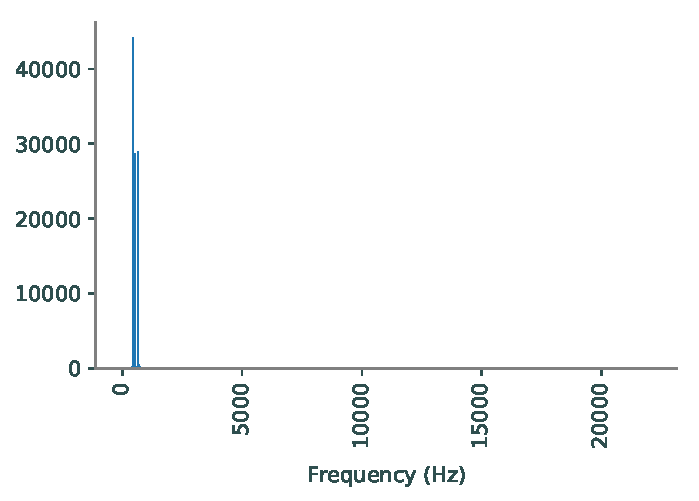
\includegraphics[scale=1.0]{figures/dft_chord.pdf}
\caption{The DFT of the minor chord.}
\label{fig:dft_chord}
\end{figure}
\end{center}

\section*{Conclusion}

If the frequencies present in a sound are already known before plotting its DFT, the plot may be interesting, but little new information is actually revealed.
Thus, the main applications of the DFT involve sounds in which the frequencies present are unknown.
One application in particular is sound filtering, which has many uses, and will be explored in greater detail in a subsequent lab.
The first step in filtering a sound is determining the frequencies present in that sound by taking its DFT.

Consider the minor chord as an example.
The plot of its DFT looks like Figure \ref{fig:dft_chord}.
This graph shows that there are three main frequencies present in the sound.
It remains to determine what exactly those frequencies are.
There are many valid ways to do this.
One possibility is to determine which indices of the array of DFT coefficients have the largest values, then scale these indices the same as the x-axis of the plot to determine to which frequencies these values correspond.
This task is explored further in the next problem.

% Problem 8: Mystery chord
\begin{problem}
The file \texttt{mystery\_sound.wav} contains an unknown chord.
Use what you have learned about the DFT to determine the individual notes present in the sound.

Hints: The function \li{np.argmax()} may be useful. Also, remember that the DFT is symmetric, meaning the last half of the array of DFT coefficients will need to be ignored.
\end{problem} 




% Additional ideas: write a method to reverse a sound? Mono vs. Stereo?

\begin{comment} % Old problem idea
\begin{problem}
Modify the \li{calculate_dft()} method so that in addition to calculating the Fourier coefficients, it also returns a list of their corresponding frequencies measured in Hertz.
\end{problem}
\end{comment}
